%
%
%
%
%
%
%
\section{Window Systems}\label{app:LFdata}
This appendix contains the details of the staggered windows of Section~\ref{sec:antipode} at a finite prime: the coverings by a hierarchy of step sizes (Appendix~\ref{app:coverings}); the staggered windows at a finite prime, which prove Theorem~\ref{thm:A} (Appendix~\ref{app:BSfinite}); their data and thresholds (Appendix~\ref{app:windowdata}); and the selection rule used for all generated window sequences (Appendix~\ref{app:steerrule}). Throughout, $p\ge5$ is prime and all window systems are instances of Proposition~\ref{prop:steer}.

\subsection{Coverings by a Hierarchy of Step Sizes}\label{app:coverings}
For product windows the covering condition (ii) of Proposition~\ref{prop:steer} is a statement about translates. In column $j$ the point $\beta+t\alpha_j$ has own entry $o=\beta_j+t$ and cross entries $\sigma_c+o\,\kappa_{c\leftarrow j}$ with $\sigma_c=\beta_c-\beta_j\kappa_{c\leftarrow j}$, and $\sigma$ runs over $\F_p^{s-1}$ as $\beta$ varies. So column $j$ satisfies (ii) if and only if for every $\sigma$ some $o\in\Wo^{(j)}$ puts every $\sigma_c+o\,\kappa_{c\leftarrow j}$ into its window $W_{c\leftarrow j}$; by Lemma~\ref{lem:volume} the column window has at least $p^{s-1}$ elements (Figure~\ref{fig:cost}).

The covering is certified by a mixed-radix hierarchy. Let the own value $o$ run through consecutive integers. If the largest step $\kappa_{c\leftarrow j}$ is at most the width of the window of its row, the translates of that window go once round the circle in a few steps; that row is the \emph{fast row}, like the last digit of an odometer. If the next step is much smaller, its row stays inside its window while the fast row goes once round, and successive rounds move it across the circle; it is a \emph{slow row}. An \emph{arc} is a set of at most $p$ consecutive residues in $\Z/p$.

\begin{lemma}[Mixed-radix covering]\label{lem:ws}
Let $k\ge1$, let $\mathbf m\in\Z^k$ with $\nu_t:=|m_t|\ge1$, and let $I_1,\dots,I_k$ be arcs. Suppose
\[
\nu_1\le|I_1|,\qquad N_1:=1+\Bigl\lceil\frac{p-|I_1|}{\nu_1}\Bigr\rceil,\qquad N_{t-1}\nu_t\le|I_t|,\quad N_t:=N_{t-1}-1+\Bigl\lceil\frac p{\nu_t}\Bigr\rceil\quad(2\le t\le k).
\]
Then for every $\sigma\in(\Z/p)^k$, every set of $N_k$ consecutive integers contains an $o$ with $\sigma+o\,\mathbf m\in I_1\times\dots\times I_k$.
\end{lemma}

\begin{proof}
By induction on $t$: every $N_t$ consecutive integers contain an $o$ with $\sigma_r+om_r\in I_r$ for all $r\le t$. \emph{Fast row.} For $N_1$ consecutive $o$, the residues $\sigma_1$ with some $\sigma_1+om_1\in I_1$ form the union of the translates $I_1-om_1$; consecutive translates are shifted by $\nu_1\le|I_1|$, so the union is an arc of $\min(p,|I_1|+(N_1-1)\nu_1)=p$ residues. \emph{Slow rows.} We may assume $m_t=\nu_t>0$. Write $I_t=\{L,\dots,L+|I_t|-1\}\bmod p$, fix an integer representative $\hat\sigma$ of $\sigma_t$, and put $o(n)=\lceil(L+np-\hat\sigma)/\nu_t\rceil$ for $n\in\Z$. For the $N_{t-1}$ integers $o(n),\dots,o(n)+N_{t-1}-1$ we have $\hat\sigma+o\nu_t\in[L+np,\,L+np+|I_t|-1]$, so $\sigma_t+o\nu_t\in I_t$. The $o(n)$ increase, are unbounded in both directions and satisfy $o(n+1)-o(n)\le\lceil p/\nu_t\rceil$; so a run of $N_t$ consecutive integers contains a whole run $o(n),\dots,o(n)+N_{t-1}-1$, which by induction contains an $o$ that is good for every $r<t$, and it is good for $t$ as well.
\end{proof}

\begin{figure}[t]
\centering
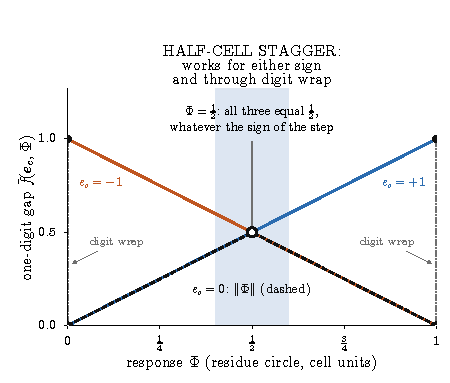
\includegraphics[width=0.48\linewidth]{fig_halfcell_v4.pdf}
\caption{The half-cell stagger: the one-digit gap $\bar f(e,\Phi)$ of Lemma~\ref{lem:antipode} for $e=+1,-1,0$. $\Phi=\frac12$ is the only response where all three agree, whatever the sign of the step; a window $\frac12\pm0.1$ is shaded (schematic).}
\label{fig:principles}
\end{figure}

\begin{figure}[t]
\centering
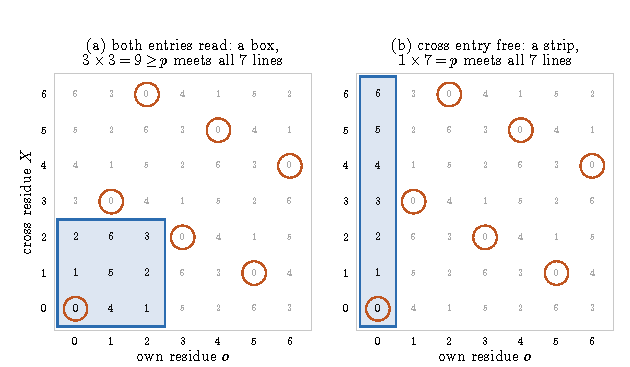
\includegraphics[width=0.66\linewidth]{fig_volume_v4.pdf}
\caption{The volume bound (Lemma~\ref{lem:volume}) for $s=2$, $p=7$, $\alpha=(1,3)$. The free digit of column $c'$ moves its responses along a line $\beta+\F_p\alpha_{c'}$, so the column window must meet every line; each pair (own, cross) is labelled by its line. (a)~A $3\times3$ box meets all $7$ lines. (b)~A strip with one own value and the full cross axis also meets all $7$ lines; an entry that the bound never reads costs nothing. Both coverings are checked exhaustively.}
\label{fig:cost}
\end{figure}

\subsection{Staggered Windows at a Finite Prime}\label{app:BSfinite}
This subsection proves Theorem~\ref{thm:A}: the bound for staggered windows at a finite prime (Lemma~\ref{lem:W}), the realization of the depth-zero crosses with the half from a power of two (Lemmas~\ref{lem:D} and~\ref{lem:R}), the staggered rule (Definition~\ref{def:BS}) and its thresholds (Proposition~\ref{prop:P0}, Theorem~\ref{thm:A3}). Throughout, $p$ is an odd prime and $C=\{c\ne\cstar\}$.

At a finite prime the windows of Section~\ref{sec:staggered} become integer intervals. We use three half-widths in row$\leftarrow$column order: $B_{C\leftarrow C}$ (into a coordinate of $C$ from another one), $B_{\star\leftarrow C}$ (the half-cell offsets) and $B_{C\leftarrow\star}$ (into $C$ from $\cstar$). For integers $A\ge0$, $M_i\ge1$ ($i\in C$) and $M_\star\ge1$, with $M:=\max_iM_i$, the \emph{staggered windows at $p$} are: in column $i\in C$, own $[-(A+M_i-1),-A]$, $W_{\star\leftarrow i}=\half+[-B_{\star\leftarrow C},B_{\star\leftarrow C}]$, $W_{j\leftarrow i}=[-B_{C\leftarrow C},B_{C\leftarrow C}]$ for $j\in C\setminus\{i\}$; in column $\cstar$, own $[-(M_\star-1),0]$ and $W_{j\leftarrow\star}=[-B_{C\leftarrow\star},B_{C\leftarrow\star}]$ for $j\in C$.

\begin{lemma}[Bound for staggered windows]\label{lem:W}
Let $s\ge2$ and suppose
\[
\text{(D)}\ A\ge(s-2)B_{C\leftarrow C}+B_{C\leftarrow\star},\qquad\text{(N)}\ A+M+(s-2)B_{C\leftarrow C}+B_{C\leftarrow\star}\le p,\quad 2B_{\star\leftarrow C}+2M_\star\le p-3 .
\]
Then $\LB(W)\ge\LB_W$, where $\LB_W^2=\min(T_\star,T_{C\star},T_2)$ with
\begin{align*}
T_\star&=\Bigl(1-\frac{M_\star}p\Bigr)^2,\qquad T_{C\star}=\Bigl(1-\frac{A+M+B_{C\leftarrow\star}}p\Bigr)^2+\Bigl(\frac{p-1-2B_{\star\leftarrow C}-2M_\star}{2p}\Bigr)^2,\\
T_2&=2\Bigl(1-\frac{A+M+(s-2)B_{C\leftarrow C}+B_{C\leftarrow\star}}p\Bigr)^2\quad(\text{omitted for }s=2).
\end{align*}
In particular, with $x:=1-((s-2)B_{C\leftarrow C}+2B_{C\leftarrow\star})/p$, $y:=\frac12-B_{\star\leftarrow C}/p$ and $A=(s-2)B_{C\leftarrow C}+B_{C\leftarrow\star}$: if $x\ge M/p$, $p(x^2+y^2-1)\ge2xM+2y(M_\star+\frac12)$ and $1-(2A+M)/p\ge1/\sqrt2$, then $\LB_W=1-M_\star/p$.
\end{lemma}

\begin{proof}
By Remark~\ref{rem:onedigit}, $f_1(1,-a)=1-(a+1)/p$ for $0\le a<p$, $f_1(1,\sigma)=(\sigma-1)/p$ for $\sigma\in[1,p-1]$, $f_1(-1,\sigma)=f_1(1,-\sigma)$, and $f_1(0,\sigma)=\max(0,\cabs\sigma-1)/p$. Fix a step $e$, $E=\operatorname{supp}e$, $k=|E\cap C|$. A moving coordinate $i\in C$ receives its own response and one cross from each other moving column, so by (D) and (N) $e_i\sigma_i\in[-(A+M-1)-(s-2)B_{C\leftarrow C}-B_{C\leftarrow\star},\,0]\subseteq[-(p-1),0]$, and $f_1(e_i,\sigma_i)\ge1-(A+M+(s-2)B_{C\leftarrow C}+B_{C\leftarrow\star})/p$; if besides $i$ only $\cstar$ moves, this improves to $1-(A+M+B_{C\leftarrow\star})/p$, and if $i$ moves alone to $1-(A+M)/p$. If $k\ge2$, two such coordinates give $T_2$. If $E=\{\cstar\}$, $f_1(1,O_\star)\ge1-M_\star/p$, which is $T_\star$. If $E=\{i\}$, the staggered coordinate does not move and receives $\half+\xi$ with $|\xi|\le B_{\star\leftarrow C}$, of centred absolute value at least $(p-1)/2-B_{\star\leftarrow C}$; the term is at least $(1-(A+M)/p)^2+((p-3-2B_{\star\leftarrow C})/(2p))^2\ge T_{C\star}$. If $E=\{i,\cstar\}$, then $e_\star\sigma_\star=\pm(\half+\xi)+O_\star$ is an integer in $[(p-1)/2-B_{\star\leftarrow C}-M_\star+1,\,(p+1)/2+B_{\star\leftarrow C}]\subseteq[1,p-1]$ by (N), so $f_1\ge(p-1-2B_{\star\leftarrow C}-2M_\star)/(2p)$, and with coordinate $i$ this is $T_{C\star}$. For the last statement, $1-(A+M+B_{C\leftarrow\star})/p=x-M/p$ and the second base of $T_{C\star}$ is at least $y-(M_\star+\frac12)/p$; since $(x-\eta_1)^2+(y-\eta_2)^2\ge x^2+y^2-2x\eta_1-2y\eta_2$, the hypothesis gives $T_{C\star}\ge1$, and $T_2\ge1$ directly.
\end{proof}

The lemma is Theorem~\ref{thm:BS} at finite $p$: with half-widths about $\varepsilon p$ and $A=(s-1)B$ its bases tend to $1-s\varepsilon$, $\frac12-\varepsilon$ and $1-2(s-1)\varepsilon$, and $x^2+y^2>1$ holds for $\varepsilon<\varepsilon_s$. Under the last statement the only loss of order $1/p$ is the own window of $\cstar$.

\emph{Realising the windows.} The fixed depth-zero crosses must lie in the windows (condition (i) of Proposition~\ref{prop:steer}): the half-cell offsets $-\kappa_{\star\leftarrow i}$ near $\half$ and all others within $O(p)$ of $0$; and every column must cover (condition (ii)). A cross $\kappa\equiv x/2$ with a small odd integer $x$ is close to $p/2$, and its multiples alternate between the two half-circles, so no mixed-radix hierarchy sees it as a small step. Its double is the small odd number $x$, and doubling the column costs a factor $2$ in the own window and nothing else.

\begin{lemma}[Doubling]\label{lem:D}
Let $\boldsymbol\xi\in\F_p^k$, let $\mathbf m\in\Z^k$ represent $2\boldsymbol\xi$, and suppose that $\mathbf m$ satisfies the hypotheses of Lemma~\ref{lem:ws} for arcs $I_1,\dots,I_k$, with number $N_k$. If $\Wo$ contains $2N_k-1$ consecutive integers, then for every $\sigma\in\F_p^k$ some $o\in\Wo$ has $\sigma+o\,\boldsymbol\xi\in I_1\times\dots\times I_k$.
\end{lemma}

\begin{proof}
$\Wo$ contains $o_0,o_0+2,\dots,o_0+2(N_k-1)$, and $\sigma+(o_0+2o')\boldsymbol\xi=(\sigma+o_0\boldsymbol\xi)+o'\mathbf m$ for $o'=0,\dots,N_k-1$; Lemma~\ref{lem:ws} applies to $\sigma+o_0\boldsymbol\xi$.
\end{proof}

By the computation at the start of Appendix~\ref{app:coverings}, this is condition (ii) for a column with steps $\boldsymbol\xi=(\kappa_{c\leftarrow c'})_{c\ne c'}$; we call such a column a \emph{doubled column}. The half itself comes from the $2$-adic valuation of the scale. By Proposition~\ref{prop:LI}(c), with the constant terms $g_c=g_c(0)$ of the multipliers,
\[
\kappa_{c\leftarrow c'}=\frac{\theta\,g_c}{g_{c'}\,\Delta_{cc'}},\qquad \Delta_{cc'}:=w'(a_{c'})\,(a_{c'}-a_c).
\]
\emph{Staggered data} $\mathcal D$ consist of distinct rational places $a_0,\dots,a_{s-1}$, a staggered coordinate $\cstar$, an order $j_1,\dots,j_{s-1}$ of $C$, and positive rationals $Q_1,\dots,Q_{s-1}$ with odd numerators and odd denominators. Let $\delta\ge0$ be the least integer with $1+2\delta\ge v_2(\Delta_{j_t\star}\Delta_{\star j_t})$ and $\delta+v_2(\Delta_{\star j_r})-v_2(\Delta_{\star j_t})-v_2(\Delta_{j_tj_r})\ge0$ for all $t\ne r$, where $v_2$ is the $2$-adic valuation, and let $L$ be the least odd positive integer such that every $L/Q_r$ and every $L\,n^\circ_{cc'}$, $c\ne\cstar$, is an integer, where $n^\circ_{cc'}$ is the value of the rational $n_{cc'}$ below at $L=1$ (it exists by the choice of $\delta$).

\begin{lemma}[The half from a power of two]\label{lem:R}
For staggered data put $g_{\cstar}=1$, $g_{j_r}=2^{1+\delta}Q_r/\Delta_{\star j_r}$ and $\theta=2^\delta LT$ with an odd integer $T$. Then $\kappa_{c\leftarrow c'}=T\,n_{cc'}$ with
\[
n_{j_t\leftarrow\star}=\frac{2^{1+2\delta}LQ_t}{\Delta_{j_t\star}\Delta_{\star j_t}}\in\Z,\qquad n_{j_t\leftarrow j_r}=2^\delta L\,\frac{Q_t}{Q_r}\cdot\frac{\Delta_{\star j_r}}{\Delta_{\star j_t}\Delta_{j_tj_r}}\in\Z,\qquad n_{\star\leftarrow j_r}=\frac{L}{2Q_r}\in\tfrac12+\Z .
\]
For every prime $p$ that divides none of the numerators and denominators of the $a_c-a_{c'}$, the $Q_r$, $L$, $T$ and $2$, the same identities hold in $\F_p$; there every $\kappa_{c\leftarrow c'}$ with $c\ne\cstar$ is the integer $Tn_{cc'}$, and each half-cell offset is $\kappa_{\star\leftarrow j_r}\equiv\half+(TL/Q_r-1)/2$, half a cell plus an integer.
\end{lemma}

\begin{proof}
Substitute $g$ and $\theta$. In the row of $\cstar$ the frame factor cancels,
\[
\frac{\theta}{g_{j_r}\Delta_{\star j_r}}=\frac{2^\delta LT}{2^{1+\delta}Q_r}=\frac{TL}{2Q_r},
\]
and $L/Q_r$ is an odd integer. The other two expressions are integers by the choice of $L$, which is possible because their $2$-adic valuations are $1+2\delta-v_2(\Delta_{j_t\star}\Delta_{\star j_t})\ge0$ and $\delta+v_2(\Delta_{\star j_r})-v_2(\Delta_{\star j_t})-v_2(\Delta_{j_tj_r})\ge0$. Modulo $p$, a half-odd rational $x/2$ is $(x+p)/2=\half+(x-1)/2$.
\end{proof}

So the half needs no congruence condition on $p$ and no root of unity, and all crosses are fixed rational multiples of one odd integer $T$.

\begin{definition}[Staggered rule]\label{def:BS}
Let $\mathcal D$ be staggered data, $\varepsilon_{C\leftarrow\star},\varepsilon_{C\leftarrow C},\varepsilon_{\star\leftarrow C}$ positive rationals (window fractions) and $u>0$ rational. At a prime $p$ as in Lemma~\ref{lem:R} with $up\ge1$:
(S1)~$T$ is the largest odd integer $\le\lfloor up\rfloor$; $\theta$ and the constants $g_c$ are those of Lemma~\ref{lem:R}, so $\kappa_{c\leftarrow c'}=Tn_{cc'}$;
(S2)~$B_\bullet=\lfloor\varepsilon_\bullet p\rfloor$ for the three half-widths, $A=(s-2)B_{C\leftarrow C}+B_{C\leftarrow\star}$, and the windows of Lemma~\ref{lem:W};
(S3)~$M_\star$ is the number $N_{s-1}$ of Lemma~\ref{lem:ws} for column $\cstar$ (steps $|\kappa_{j\leftarrow\star}|$ in decreasing order, arcs $[-B_{C\leftarrow\star},B_{C\leftarrow\star}]$), and $M_i=2N^{(i)}-1$, where $N^{(i)}$ is the number of Lemma~\ref{lem:ws} for the doubled column $i$ (steps $|2\kappa_{c\leftarrow i}|$ in decreasing order, the half-cell offset contributing the odd integer $|TL/Q_r|$; arcs of the rows);
(S4)~any selection rule (Appendix~\ref{app:steerrule}).
\end{definition}

The rule is a fixed computation of $O(s^2)$ integer operations plus the selection of the free digits; it involves no search and no covering check. It satisfies the hypotheses of Proposition~\ref{prop:steer} and Lemmas~\ref{lem:ws}, \ref{lem:D} and~\ref{lem:W} for all large $p$ as soon as its limit as $p\to\infty$ does. For a column, let $\bar\nu_1\ge\dots\ge\bar\nu_{s-1}>0$ be its steps divided by $p$ in the limit, $\bar\nu=u|n_{c\leftarrow\star}|$ in column $\cstar$ and $\bar\nu=2u|n_{c\leftarrow i}|$ in a doubled column $i\in C$, and let $\lambda_t=2\varepsilon_\bullet$ be the window fraction of the corresponding row. The data satisfy the \emph{limit hierarchy} if in every column
\[
\bar\nu_1<\lambda_1,\qquad \bar N_{t-1}\,\bar\nu_t<\lambda_t\quad(2\le t\le s-1),\qquad \bar N_1=2+\frac{1-\lambda_1}{\bar\nu_1},\quad \bar N_t=\bar N_{t-1}+\frac1{\bar\nu_t},
\]
and the fixed depth-zero crosses lie strictly inside their windows: $u|n_{c\leftarrow c'}|<\varepsilon_\bullet$ for $c\ne\cstar$ and $2u|n_{\star\leftarrow i}|<2\varepsilon_{\star\leftarrow C}$. These are the limits of the hypotheses of Lemma~\ref{lem:ws} and of condition (i).

\begin{proposition}[Threshold]\label{prop:P0}
For the staggered rule with given data there are an explicit finite conjunction $\mathcal P(p)$ of inequalities between rational functions of a real variable $p$ and an explicit function $M_\star^+(p)$ such that (a) and (b) hold; if moreover the data satisfy the limit hierarchy, $0<\varepsilon_{\star\leftarrow C}<\frac12$, and $x=1-(s-2)\varepsilon_{C\leftarrow C}-2\varepsilon_{C\leftarrow\star}$ and $y=\frac12-\varepsilon_{\star\leftarrow C}$ satisfy $x^2+y^2>1$ and $1-2(s-2)\varepsilon_{C\leftarrow C}-2\varepsilon_{C\leftarrow\star}>1/\sqrt2$, then also (c) holds.
\begin{enumerate}
\item[(a)] At every prime $p$ as in Lemma~\ref{lem:R} with $\mathcal P(p)$, the staggered rule satisfies (i) and (ii) of Proposition~\ref{prop:steer} and the hypotheses of Lemma~\ref{lem:W} including its last statement, with $M_\star\le M_\star^+(p)$.
\item[(b)] $\mathcal P(p)$ implies $\mathcal P(p')$ for every $p'\ge p$, and $M_\star^+$ is non-increasing.
\item[(c)] $\mathcal P(p)$ holds for all large $p$.
\end{enumerate}
Consequently, if $\mathcal P(p_0)$ holds, then for every prime $p\ge p_0$ as in Lemma~\ref{lem:R} the staggered rule gives a digital $(0,s)$-sequence over $\F_p$ with $\sep{P_{sK}}\ge1-C''/p$ for every $K$, where $C'':=M_\star^+(p_0)$; under the hypotheses of (c) such a $p_0$ exists.
\end{proposition}

The list $\mathcal P$ and the proof are in Appendix~\ref{app:windowdata}; any $p_0$ with $\mathcal P(p_0)$ is a valid threshold, certified by one exact rational evaluation.

\begin{theorem}[The staggered rule in dimension three]\label{thm:A3}
Let $s=3$ and take the staggered data with the Faure places $(0,1,2)$, $\cstar=0$, order $(1,2)$ and $(Q_1,Q_2)=(7,3)$; then $\delta=2$, $L=21$, $\theta=84T$, $g=(1,-56,6)$, and
\[
\kappa_{1\leftarrow0}=2352T,\quad\kappa_{2\leftarrow0}=-126T,\quad\kappa_{0\leftarrow1}=\tfrac32T,\quad\kappa_{0\leftarrow2}=\tfrac72T,\quad\kappa_{1\leftarrow2}=-392T,\quad\kappa_{2\leftarrow1}=-9T.
\]
With $u=891/78\,400\,000$ and $(\varepsilon_{C\leftarrow\star},\varepsilon_{C\leftarrow C},\varepsilon_{\star\leftarrow C})=(\frac{27}{1000},\frac1{200},\frac1{10})$, the staggered rule gives for every prime $p\ge1.97\cdot10^7$ a quasi-uniform digital $(0,3)$-sequence over $\F_p$ with $\sep{P_{3K}}\ge1-742/p$ for every $K\ge1$.
\end{theorem}

\begin{proof}
The six crosses are Lemma~\ref{lem:R} (the excluded primes are $2$, $3$, $7$). The condition $\mathcal P(p_0)$ holds at $p_0=19\,673\,600$, with $M_\star^+(p_0)=742.355\ldots$, by one exact rational evaluation (proof${}^\star$); as $M_\star$ is an integer, $M_\star\le742$. Lemma~\ref{lem:prefix} gives quasi-uniformity.
\end{proof}

The half-cell offsets are $\frac32T$ and $\frac72T$; in column $\cstar$ the fast row has the step $\kappa_{1\leftarrow0}\approx0.027p$; the first-order deficit $742$ is the size of the own window of $\cstar$.

\begin{remark}[Below the threshold]\label{rem:A3range}
The hypotheses of Proposition~\ref{prop:steer} and Lemma~\ref{lem:W} for this rule are integer conditions at each prime. Checked at all $1\,035\,877$ primes in $[3\cdot10^6,1.97\cdot10^7]$ by a program that computes the crosses in $\F_p$ from the constants $g_c$ (not from Lemma~\ref{lem:R}), they hold with $(1-\LB_W)p\le779$ (c.a.). So the staggered rule gives $\sep{P_{3K}}\ge1-779/p$ for every prime $p\ge3\cdot10^6$.
\end{remark}

\begin{proof}[Proof of Theorem~\ref{thm:A}]
Take any staggered coordinate, the natural order of $C$, uniform window fractions $\varepsilon<\varepsilon_s$, and $Q_r=R^r$ with an odd integer $R$. By Lemma~\ref{lem:R}, $n_{cc'}=2^\delta L\,R^{e}f_{cc'}$, where $f_{cc'}$ does not depend on $R$ and $e=t$ in row $j_t$ of column $\cstar$, $e=t-r$ in row $j_t$ of column $j_r$, and $e=-r$ for the half-cell offset of column $j_r$. The exponents in one column are distinct, so for $R$ large consecutive steps of every column differ by a factor at least $1+1/\varepsilon$, and the largest step of every column $i\in C$ (exponent at most $s-2$) is smaller than the largest step of column $\cstar$ (exponent $s-1$). Choose $u$ so that the latter is $(1-\eta)\varepsilon$ with $0<\eta<1$. Then $\bar\nu_1<\lambda_1=2\varepsilon$ in every column, the fixed depth-zero crosses are strictly inside their windows, and for $t\ge2$
\[
\bar N_{t-1}\bar\nu_t\le2\bar\nu_t+\sum_{r<t}\frac{\bar\nu_t}{\bar\nu_r}\le2\bar\nu_t+\sum_{j\ge1}\Bigl(1+\frac1\varepsilon\Bigr)^{-j}=2\bar\nu_t+\varepsilon<2\varepsilon=\lambda_t,
\]
because $2\bar\nu_t\le4\varepsilon/(1+1/\varepsilon)<\varepsilon$ for $\varepsilon<\frac13$. So the limit hierarchy holds. With uniform widths, $x=1-s\varepsilon$ and $y=\frac12-\varepsilon$, and $x^2+y^2>1$ follows from $\varepsilon<\varepsilon_s$ (proof of Theorem~\ref{thm:BS}); as $y^2<\frac14$, this forces $(1-s\varepsilon)^2>\frac34$, hence $1-2(s-1)\varepsilon>1-(2-\sqrt3)>1/\sqrt2$. Proposition~\ref{prop:P0} gives $p_0(s)$ and $C''_s$; the primes excluded in Lemma~\ref{lem:R} are finitely many, and Lemma~\ref{lem:prefix} gives quasi-uniformity.
\end{proof}

For $s=4$ (staggered coordinate $0$, $R=153$, $\varepsilon=7/250$) Proposition~\ref{prop:P0} gives $p_0=1.44\cdot10^{16}$ and $C''_4=32\,044$, and for $s=5$ (staggered coordinate $4$, $R=99$, $\varepsilon=23/1000$) $p_0=1.98\cdot10^{21}$ and $C''_5=2.73\cdot10^9$ (exact rational evaluations, proof${}^\star$; Table~\ref{tab:BSdata}). Coverings of lattice type instead of one shared hierarchy of step sizes are a possible route to lower thresholds (Section~\ref{sec:open}). Figure~\ref{fig:bsgeom} shows the geometry of Section~\ref{sec:staggered} in a staggered window system at a moderate prime, with coverings checked exactly instead of by the rule.

\begin{figure}[t]
\centering
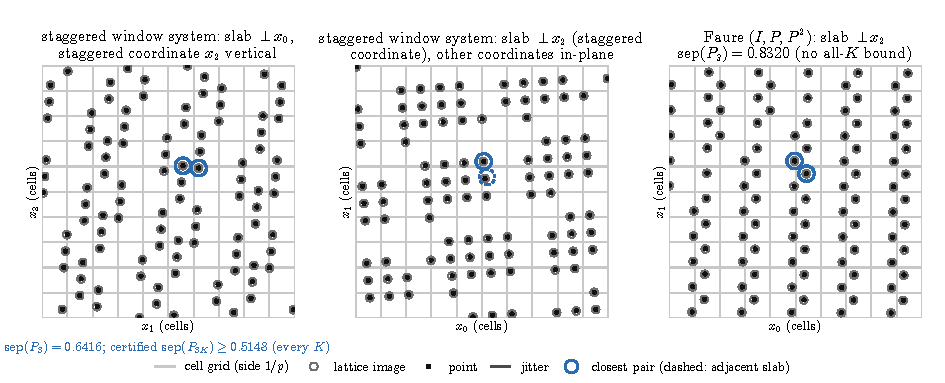
\includegraphics[width=\linewidth]{fig_bs_slab_v4.pdf}\\[2pt]
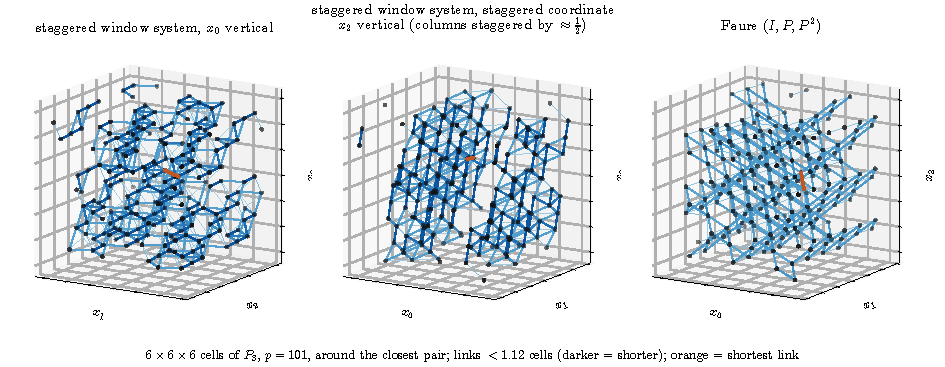
\includegraphics[width=\linewidth]{fig_bs_3d_v4.pdf}
\caption{Staggered windows in dimension three: a staggered window system at $p=101$ with exactly checked coverings (certified $\sep{P_{3K}}\ge0.5148$ for every $K$) and one admissible choice of the free digits. Top: slabs of $P_3$ one cell thick, $10\times10$ cells around the closest pair. Left, staggered coordinate vertical: the columns are staggered by about half a cell. Middle, orthogonal to the staggered coordinate: the coordinates of $C$ are pushed together and wrap around along staircases. Right, Faure $(I,\Pas,\Pas^2)$. Exact $\sep{P_3}$: $0.6416$, and $0.8320$ for Faure, which has no bound for all levels. Bottom: $6\times6\times6$ cells around the closest pair, links shorter than $1.12$ cells (darker $=$ shorter, orange $=$ shortest), in the same three views.} %
\label{fig:bsgeom}
\end{figure}

\subsection{Staggered Data and Thresholds}\label{app:windowdata}
\emph{Staggered data.} Table~\ref{tab:BSdata} gives the three staggered rules of Theorems~\ref{thm:A3} and~\ref{thm:A}. In each, $\theta=2^\delta LT$ and $\kappa_{c\leftarrow c'}=Tn_{cc'}$ with the rationals $n_{cc'}$ of Lemma~\ref{lem:R}; for $s=4,5$ the window fractions are uniform, $\varepsilon_{C\leftarrow\star}=\varepsilon_{C\leftarrow C}=\varepsilon_{\star\leftarrow C}=\varepsilon$, with $u=\frac{999}{1000}\,\varepsilon/\max_t|n_{j_t\leftarrow\star}|$, which puts the step of the fast row of column $\cstar$ just inside its window.

\begin{table}[t]
\centering
\small
\caption{The staggered data: Faure places $(0,1,\dots,s-1)$, staggered coordinate $\cstar$, order of $C$, the rationals $Q_r$, the $2$-adic data $\delta$, $L$ and the constants $g_c$ of Lemma~\ref{lem:R} (for $c=0,\dots,s-1$), window fractions, $u$, the threshold $p_0$ (exact bisection endpoint, rounded up in the last digit shown) and the first-order deficit $C''=M_\star^+(p_0)$ (rounded up).}
\label{tab:BSdata}
\begin{tabular}{@{}lccc@{}}
\toprule
& $s=3$ (Thm.~\ref{thm:A3}) & $s=4$ & $s=5$\\
\midrule
$\cstar$; order & $0$; $(1,2)$ & $0$; $(1,2,3)$ & $4$; $(0,1,2,3)$\\
$Q_r$ & $(7,3)$ & $153^r$ & $99^r$\\
$\delta$; $L$ & $2$; $21$ & $2$; $3\,581\,577$ & $5$; $96\,059\,601$\\
$g_c$ & $(1,-56,6)$ & $(1,612,-46818,1591812)$ & $(-66,34848,-7762392,$\\
& & & $1024635744,1)$\\
$(\varepsilon_{C\leftarrow\star},\varepsilon_{C\leftarrow C},\varepsilon_{\star\leftarrow C})$ & $(\frac{27}{1000},\frac1{200},\frac1{10})$ & $\varepsilon=\frac7{250}$ & $\varepsilon=\frac{23}{1000}$\\
$u$ & $891/78\,400\,000$ & $259/(1.1730858534\cdot10^{16})$ & $851/(4.860548184640896\cdot10^{21})$\\
$p_0$ & $19\,673\,600$ & $1.43146\cdot10^{16}$ & $1.97832\cdot10^{21}$\\
$C''$ & $742.356$ & $32044.14$ & $2.72224\cdot10^9$\\
\bottomrule
\end{tabular}
\end{table}

\emph{The predicate $\mathcal P(p)$.} Fix staggered data and a real $p>0$. For a column, sort its steps by $|n|$ in decreasing order, $n_1,\dots,n_{s-1}$; let $k=1$ for column $\cstar$ and $k=2$ for a column $i\in C$ (Lemma~\ref{lem:D}; there the half-cell offset contributes $2|n_{\star\leftarrow i}|=L/Q_r$), and let $\lambda_t=2\varepsilon_\bullet$ be the window fraction of the row of step $t$. Put
\[
\nu_t^-=k|n_t|(up-2),\qquad\nu_t^+=k|n_t|\,up,\]\[N_1^+=2+\max\Bigl(0,\frac{p-(p\lambda_1-1)}{\nu_1^-}\Bigr),\qquad N_t^+=N_{t-1}^++\frac p{\nu_t^-},
\]
let $M_\star^+$ be $N_{s-1}^+$ of column $\cstar$ and $M^+$ the maximum of $2N_{s-1}^+-1$ over the columns $i\in C$, and let $x$, $y$ be as in Proposition~\ref{prop:P0}. Then $\mathcal P(p)$ is the conjunction of
(P1)~$up>2$;
(P2)~in every column, $\nu_1^+\le p\lambda_1-1$ and $N_{t-1}^+\nu_t^+\le p\lambda_t-1$ for $2\le t\le s-1$;
(P3)~$|n_{c\leftarrow c'}|\,up\le\varepsilon_\bullet p-1$ for every cross with $c\ne\cstar$, where $\varepsilon_\bullet$ is the fraction of its window, and $|2n_{\star\leftarrow i}|\,up\le2(\varepsilon_{\star\leftarrow C}p-1)-1$ for every half-cell offset;
(P4)~$x^2+y^2>1$ and $p\,(x^2+y^2-1)\ge2xM^++2y\,(M_\star^++\frac12)$;
(P5)~$z:=1-2(s-2)\varepsilon_{C\leftarrow C}-2\varepsilon_{C\leftarrow\star}-M^+/p\ge0$ and $2z^2\ge1$;
(P6)~$\bigl(2(s-2)\varepsilon_{C\leftarrow C}+2\varepsilon_{C\leftarrow\star}\bigr)p+M^++2\le p-1$, $2\varepsilon_{\star\leftarrow C}\,p+2M_\star^++2<p-1$ and $x>M^+/p$.
At a prime $p$, $T\in(up-2,up]$ and every arc of row $t$ has at least $p\lambda_t-1$ elements, so (P2) gives the hypotheses of Lemma~\ref{lem:ws} (with $N_t\le N_t^+$), (P3) condition (i) of Proposition~\ref{prop:steer}, and (P4)--(P6) the hypotheses of Lemma~\ref{lem:W} including its last statement ((P5) is $z\ge1/\sqrt2$; under (P6) the difference of the two sides of $p(x^2+y^2-1)\ge2xM+2y(M_\star+\frac12)$ increases in $x$ and $y$).

\begin{proof}[Proof of Proposition~\ref{prop:P0}]
$\mathcal P$ is obtained from the hypotheses by four substitutions: $T\in(up-2,up]$, so every step lies in $[k|n|(up-2),\,k|n|up]$; every arc has at least $p\lambda_t-1$ elements; $\lceil z\rceil\le z+1$ in the recursion of Lemma~\ref{lem:ws}, which bounds the numbers $N_t$ by the sums $N_t^+$, and hence $M_\star$, $M$ by $M_\star^+$, $M^+$; and Lemma~\ref{lem:W} is replaced by its last statement. Since $T$ is common to all entries, sorting the steps of a column by size is sorting by $|n|$, independently of $p$. (a) is the statement that each substituted inequality implies the original one; for the half-cell offsets, $2\kappa_{\star\leftarrow i}=TL/Q_r$ is an odd integer and $-\kappa_{\star\leftarrow i}\equiv\half-(TL/Q_r+1)/2$. (b) Each $N_t^+$ is a sum of terms that decrease in $p$ for $up>2$, and after division by $p$ every inequality of $\mathcal P$ has the form ``non-increasing $\le$ non-decreasing''. (c) The hypotheses give $\varepsilon_{\star\leftarrow C}<\frac12$ and $2(s-2)\varepsilon_{C\leftarrow C}+2\varepsilon_{C\leftarrow\star}<1$, so every window fraction is below $\frac12$, $\lambda_1<1$ and the maximum in $N_1^+$ is its second term. As $p\to\infty$, $N_t^+\to\bar N_t$ and $M^+/p\to0$, so the strict inequalities of the limit hierarchy give $\mathcal P(p)$ for large $p$. The bound is Proposition~\ref{prop:steer} with Lemma~\ref{lem:W}: $\LB(W)\ge1-M_\star/p\ge1-M_\star^+(p_0)/p$.
\end{proof}

By Proposition~\ref{prop:P0}(b), $\mathcal P$ is monotone, and a bisection in exact rational arithmetic gives a point $p_0$ where $\mathcal P(p_0)$ holds: $19\,673\,600$, $14\,314\,526\,192\,182\,751$ and $1\,978\,313\,734\,082\,584\,379\,393$ for $s=3,4,5$. Theorems~\ref{thm:A3} and~\ref{thm:A} round these up to $1.97\cdot10^7$, $1.44\cdot10^{16}$ and $1.98\cdot10^{21}$; since the own size $M_\star$ is an integer at most $M_\star^+(p_0)$, the first-order deficits are at most $742$, $32\,044$ and $2.73\cdot10^9$ (for $s=4$, $\mathcal P$ fails at $1.43\cdot10^{16}$).

\subsection{The Selection Rule}\label{app:steerrule}
For reproducibility we fix one deterministic choice of the free digits; the window sequences of the figures use it.

\begin{remark}[A greedy selection rule]\label{rem:steerrule}
In all our window systems the own windows are integer intervals $[\mathrm{lo}_c,\mathrm{hi}_c]\subseteq[-(p-1),0]$. Rank an admissible own value $o$ (its representative in the interval) by its distance $|2o-\mathrm{lo}_c-\mathrm{hi}_c|$ from the centre, ties to the larger $o$. At depth $1$ the responses are $D(1)$, with the own values on the diagonal and $-\kappa_{c\leftarrow c'}$ off it, and the admissible depth-one own values of different columns are independent. The rule chooses, over all combinations of admissible depth-one own values, one that maximises $\LBact_1$, ties broken by the ranking, column by column; at every depth $l\ge2$ it takes the best-ranked admissible own value of each column. It uses no look-ahead and no randomness, so a sequence is determined by its places, $\theta$, the $\lambda_c$ and the windows. By Proposition~\ref{prop:steer} it has the same bound $\min(1,\LB(W))$ at every full level as any other rule, and in addition $\sep{P_s}\ge\min(1,\LBact_1)$ with the best possible depth-one choice. That it maximises $\sep{P_s}$ or $\sep{P_{sK}}$ is not claimed; among the selection rules we compared on $\sep{P_3}$, it was within $10^{-3}$ of the best in $32$ of $35$ cases and never below $0.966$ of it, while rules that look at one column at a time lost up to $40\%$ at some primes.
\end{remark}
